%
% section 7.2.2
%
\subsection{Διαχείριση Σφαλμάτων}

Για να λειτουργεί σωστά το δίκτυο, θα πρέπει να φροντίζουμε να λειτουργούν σωστά τα επιμέρους στοιχεία του. Σε ένα δίκτυο μπορεί να συμβαίνουν τόσο βλάβες / σφάλματα όσο και λάθη.

\begin{inthebox}
\textbf{Σημείωση:} Το βιβλίο εδώ αναφέρει το ``σφάλμα'' ως συνώνυμο της ``βλάβης''. Στην πραγματικότητα ``σφάλμα'' και ``λάθος'' είναι συνώνυμες λέξεις στα ελληνικά. Στην ξένη βιβλιογραφία η βλάβη αναφέρεται ως \textbf{fault} ενώ το λάθος ως \textbf{error} και είναι πράγματι διαφορετικές έννοιες όπως θα δείτε στους παρακάτω ορισμούς.\\
\end{inthebox}

\begin{figure}[!ht]
 \centering
 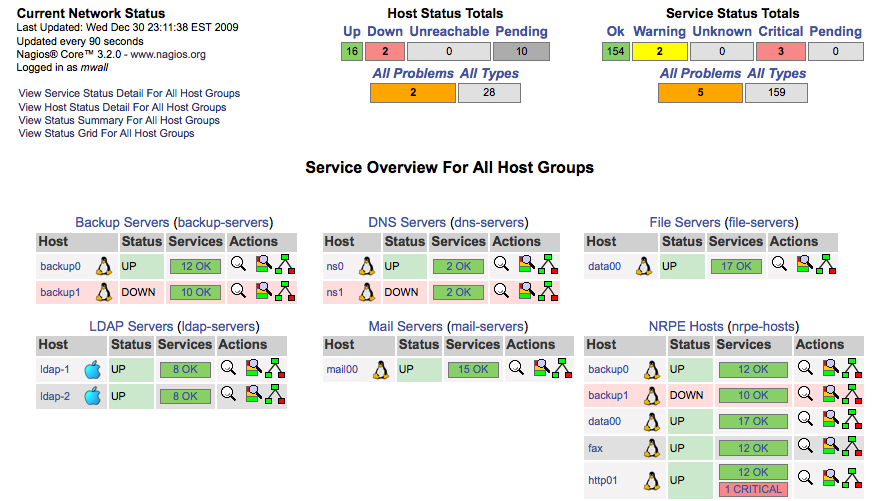
\includegraphics[width=0.95\textwidth]{images/chapter7/7-3}
 \caption {\textsl{Σύστημα Διαχείρισης Δικτύου (NMS)}}
 \label{7-3}
\end{figure}

\emph{Βλάβη ή σφάλμα} είναι μια μη φυσιολογική κατάσταση που απαιτεί την προσοχή του διαχειριστή και την άμεση διόρθωση του. Μια βλάβη συνεπάγεται μη σωστή λειτουργία ή μεγάλο αριθμό λαθών και προβλημάτων. Για παράδειγμα ένα καλώδιο δικτύου το οποίο δεν κάνει καλή επαφή μπορεί να προκαλεί διακοπές στο δίκτυο ή μεγάλο αριθμό από λανθασμένα bit.

\emph{Λάθος} είναι ένα μεμονωμένο γεγονός το οποίο συνήθως δεν συνεπάγεται διακοπή της επικοινωνίας. Σε πολλές περιπτώσεις το δίκτυο μπορεί να διορθώνει αυτόματα λάθη που οφείλονται σε τυχαία γεγονότα (π.χ. παρεμβολή σε ένα καλώδιο δικτύου μπορεί να προκαλέσει τη λανθασμένη λήψη κάποιων bit) χρησιμοποιώντας μηχανισμούς ελέγχου που περιέχονται στα ίδια τα πρωτόκολλα (θυμηθείτε π.χ. ότι το TCP έχει άθροισμα ελέγχου και τη δυνατότητα να μεταδώσει ξανά τα χαλασμένα τμήματα).

Ο εντοπισμός ενός σφάλματος (βλάβης) μπορεί να γίνει έμμεσα, με την \emph{παρατήρηση ενδείξεων} από την κίνηση και τη συμπεριφορά του δικτύου σε πραγματικό χρόνο (παρατηρούμε ότι μια σελίδα που κανονικά ανοίγει πολύ γρήγορα καθυστερεί υπερβολικά, ή ότι ένας κοινόχρηστος φάκελος στο δίκτυο δεν ανταποκρίνεται) είτε σε \emph{μορφή συναγερμού (alarm)} εφόσον έχουμε εγκαταστήσει ένα Σύστημα Διαχείρισης Δικτύου (σχήμα \ref{7-3}). 

Σε περίπτωση σφάλματος, υπάρχουν συγκεκριμένα βήματα που πρέπει να ακολουθήσουμε για την αντιμετώπιση του και γενικά ονομάζονται \emph{Κύκλος Επεξεργασίας Διαχείρισης Σφαλμάτων, Fault Management Process Cycle}. Τα συνήθη βήματα είναι τα παρακάτω:

\begin{itemize}
\item \textbf{Να προσδιοριστεί το σφάλμα}, να βρεθεί δηλαδή τι είδους σφάλμα είναι και από που μπορεί να προέρχεται.
\item \textbf{Να εντοπιστεί το σφάλμα}, ώστε να ανακαλυφθεί σε πιο σημείο του δικτύου βρίσκεται
\item \textbf{Να απομονωθεί το υπόλοιπο του δικτύου}, ώστε να λειτουργεί χωρίς να εμποδίζεται από το σφάλμα
\item \textbf{Να αναδιαμορφωθεί το δίκτυο} ώστε να μπορεί να λειτουργεί όσο το δυνατόν καλύτερα για όσο υπάρχει ακόμα το σφάλμα
\item \textbf{Να γίνει έλεγχος και ανάλυση των ενδείξεων} ώστε να κατανοηθεί καλύτερα η αιτία και να δοθεί μια καλύτερη εξήγηση της πηγής του σφάλματος
\item \textbf{Να επισκευαστεί ή να αντικατασταθεί} το υλικό ή το λογισμικό που προκάλεσε τη βλάβη ώστε το δίκτυο να επανέλθει στην προηγούμενη του λειτουργική κατάσταση
\item \textbf{Να παρακολουθηθεί το δίκτυο} από το διαχειριστή για ένα προκαθορισμένο χρονικό διάστημα ώστε να επιβεβαιωθεί η σωστή λειτουργία του και να είμαστε σίγουροι ότι το σφάλμα επιλύθηκε επιτυχώς
\end{itemize}

Η επίδραση που έχει ένα σφάλμα στο δίκτυο μπορεί να μετριαστεί αν έχουμε φροντίσει να υπάρχουν για παράδειγμα πολλαπλές (εναλλακτικές) διαδρομές που να ενώνουν δυο σημεία επικοινωνίας (αλλαγή διαδρομής). Όσο αφορά το δικτυακό υλικό, μπορούμε να διαθέτουμε πολλαπλές δικτυακές συσκευές για την ίδια εργασία ώστε να αναλαμβάνει κάποια άλλη το φορτίο του δικτύου σε περίπτωση βλάβης. 

Για παράδειγμα, σε πολλούς εξυπηρετητές δικτύου χρησιμοποιούμε συστήματα mir\-ror (καθρέπτη) στους σκληρούς δίσκους: τα δεδομένα μας αποθηκεύονται ταυτόχρονα σε περισσότερους από ένα δίσκους και το σύστημα μπορεί να συνεχίσει να λειτουργεί κανονικά ακόμα και μετά από απώλεια ενός ή περισσότερων δίσκων. Στην περίπτωση αυτή βέβαια ειδοποιείται ο διαχειριστής για να αντικαταστήσει το χαλασμένο δίσκο το συντομότερο δυνατόν.

